\chapter{Domain analysis}
\label{chap:Domain analysis}
In this chapter I will describe the requirements for the system as they have been decided to be in collaboration with Kristian. I will describe what users will be in the system, and why they are there.

I will also set up both functional and non functional requirements, and use some of the functional requirements to create use cases, describing how the system should work in the described cases.

After this I create a domain model, describing the domain of the system, and use some time explaining how it should be read, as not all the notations are standards, but I feel they need to be there in order to give the desired information.

I will in the end create a few mockups to give an idea of how the front-end could look based on the data given from back-end.

\section{Requirements}
\label{sec:Requirements}
In order for me to know what is expected of the system I have spoken with Kristian W. Larsen, and together we have come up with some requirements for the system. This includes what users should be in the system, as well as what those users can do. We also talked about some of the views that are important to have for the CRM to be usable, and what annoys him in the existing CRM's, so that this one will be more to IT minds needs.

\subsection{Users}
\label{sub:Users}

One of the basic requirements are the users that the system will support. Ideally the following three user types should be supported, each with the rights of the previous, as well as some rights of their own.

\begin{itemize}
  \item Super
  \item Executive
  \item Standard
\end{itemize}

The executive does not have any special rights compared to the standard user
initially, but they my have pre-designed overviews, because their role in the
system is to gain an overview of the all the users in a department or user
group. They can of course also do the same as a standard user, such as create
people and companies. In the future they may gain privileges that the standard
user is not supposed to have, but for now that will not be the case.

One could argue that it is pointless to have that user at this point since it cannot do anything special, but the primary argument is that IT minds, and a lot of others have this structure in delegation of responsibility, and if in the future we decide that there is some information that the executives should have access to but the normal users should not, the setup is already in place, and the super user will not have to reassign all the users who are supposed to be executives.

This leads to the things the super user can do. This include invitation of users, and assignment of groups and roles. They should also be able to define what groups are available, as well as departments and activity categories. It will also be the super admin who defines states and their percentage value.

A final thing that users should have is production goals, this means that the super user should be able to assign a goal for the user to sell for every month. But because this value may increase it should be in a way so that the assignment is associated with a month and year, and it will run until the next assigned value, which then takes over from that month.

This is a requirement because it gives the users something to aim fore, and allows for a visualization of earnings versus goals, which will be discussed in section~\ref{sub:Visualization}.

\subsection{Resources}
\label{sub:Resources}

A theme with a lot of the requirements was the desire to be able to customize,
instead of having the system enforce things on the users. The things that should
be customizable is categories, departments, stages and the like. Generally
things that tag something, and that may carry a value with it, such as stage,
which is supposed to have a percentage of certainty for an opportunity. Letting
the super user make the stages them selves also allows them to set what the
stage actually means, allowing a system that suites the individual company's way
of working better. 

The customization should only be something that the super user can create, as to avoid too many things that essentially mean the same to show up. In the case of an opportunity the tag that a stage shows may be fitting while the value is not, therefore it is also desired that the creator of the opportunity can overrule the suggested value that the stage carries to fit better with each individual opportunity.

The system should keep track of opportunities which are possible deals, and
deals that are won. An opportunity needs to contain some information such as who
is responsible for it, and who the deal is with, as well as how much it will
earn. A full list of what an opportunity should contain can be seen in
figure~\ref{fig:domain_model}.

The primary reason for IT minds to want a new CRM is that most other CRM's
front-load the earning from an opportunity, resulting in a task that that will
earn a lot of money, but also takes up a lot of resources looking like it has no
impact on any of the months after the first. This is not how it works in
reality, as the company who hires eg. IT minds to work for a couple of months
pay a little bit every month instead of everything all at once. The solution to
this is mostly in regards to data visualization, where we need to keep track of
the span of an opportunity, and what it will earn over that period, this should
then be divided out over the span of the opportunity, also meaning that the
earnings of a user is based on the same, since it needs to be possible to set
goals for the user on a per month basis. 

Since an opportunity is a bigger thing, and there will be a lot of work related to a single one, I also need a way to keep track of smaller tasks, such as making a call, or going to a meeting. This is where an activity comes in to the picture. An activity should be able to be several things defined by the super admin, but the primary thing that it does is define a task for a user to do. The task could be to send an email, or make a call, or go to a conference. Because these things don't take the same amount of time a category for them can have a value, so it can be visualized what the users are using their time on. This is useful as right now IT minds ports the number of activity for all the users to a spread sheet, and graphs from there, but if the system could do that for them some inconvenience would be saved.

\subsection{Visualization}
\label{sub:Visualization}
For the visualization the primary goal if that a user should be able to see the different types of data illustrated in graphs. This means that a thing such as the data of what a user have earned in a period, versus their goal in that given period. Ideally the graph should be made in such a way that some view based settings can be given, and an executive would be able to get an overview over the sum of all the goals versus the sum of all the sales that the users have done. It should be possible to filter it both on a per department, and user bases.

The view settings that a user chooses should be saved to the database, so that they do not have to reset it every tine they visit that same page, as in the long run that would take up a lot of their time.

A feature that has been requested is that instead of having a sale of eg. 1.500.000 kr. in one month be set as that user having sold for that amount in that month, but instead have the value spaced out over the period that the project will run, as this will illustrate in a more clear way how the sales personal is able to generate work, and allocate the resources of the company.

\subsection{Functional and nonfunctional requirements}
\label{sub:Functional and nonfunctional requirements}

\subsubsection{Functional requirements}
\label{subs:Functional requirements}
\begin{enumerate}[label=\textbf{F\arabic*}]
  \item Super invites new users
  \item Super manages users
  \item Login with email/password combination
  \item Customizable categories, groups and departments
  \item Creation of opportunities
  \item Update opportunities
  \item Creation of companies and their employees
  \item Management of companies and employees
  \item Creation of activities
  \item Manage activity
  \item Possibility of making a recap on an activity
  \item Measurability of activities
  \item Filters for visualization
  \item Overview of goals, per user and globally
  \item Overview of production
  \item Search for items
\end{enumerate}

\subsubsection{Non functional requirements}
\label{subs:Non functional requirements}
\begin{enumerate}[label=\textbf{NF\arabic*}]
  \item Should keep user information secure
  \item Should be accessible 98\% of the time
  \item Communication should happen securely
  \item Visual design should be easily updatable
\end{enumerate}


\section{Use cases}
\label{sec:Use cases}
From the requirements of section~\ref{sec:Requirements} I have created a use case diagram, to help identify the use cases that is in the project, as can be seen in Figure~\ref{fig:usecase_diagram}. To help create the diagram I used an Actor - Goal list, that can be seen in Appendix~\ref{app:actor-goal}.

\begin{figure}[!htb]
  \centering
  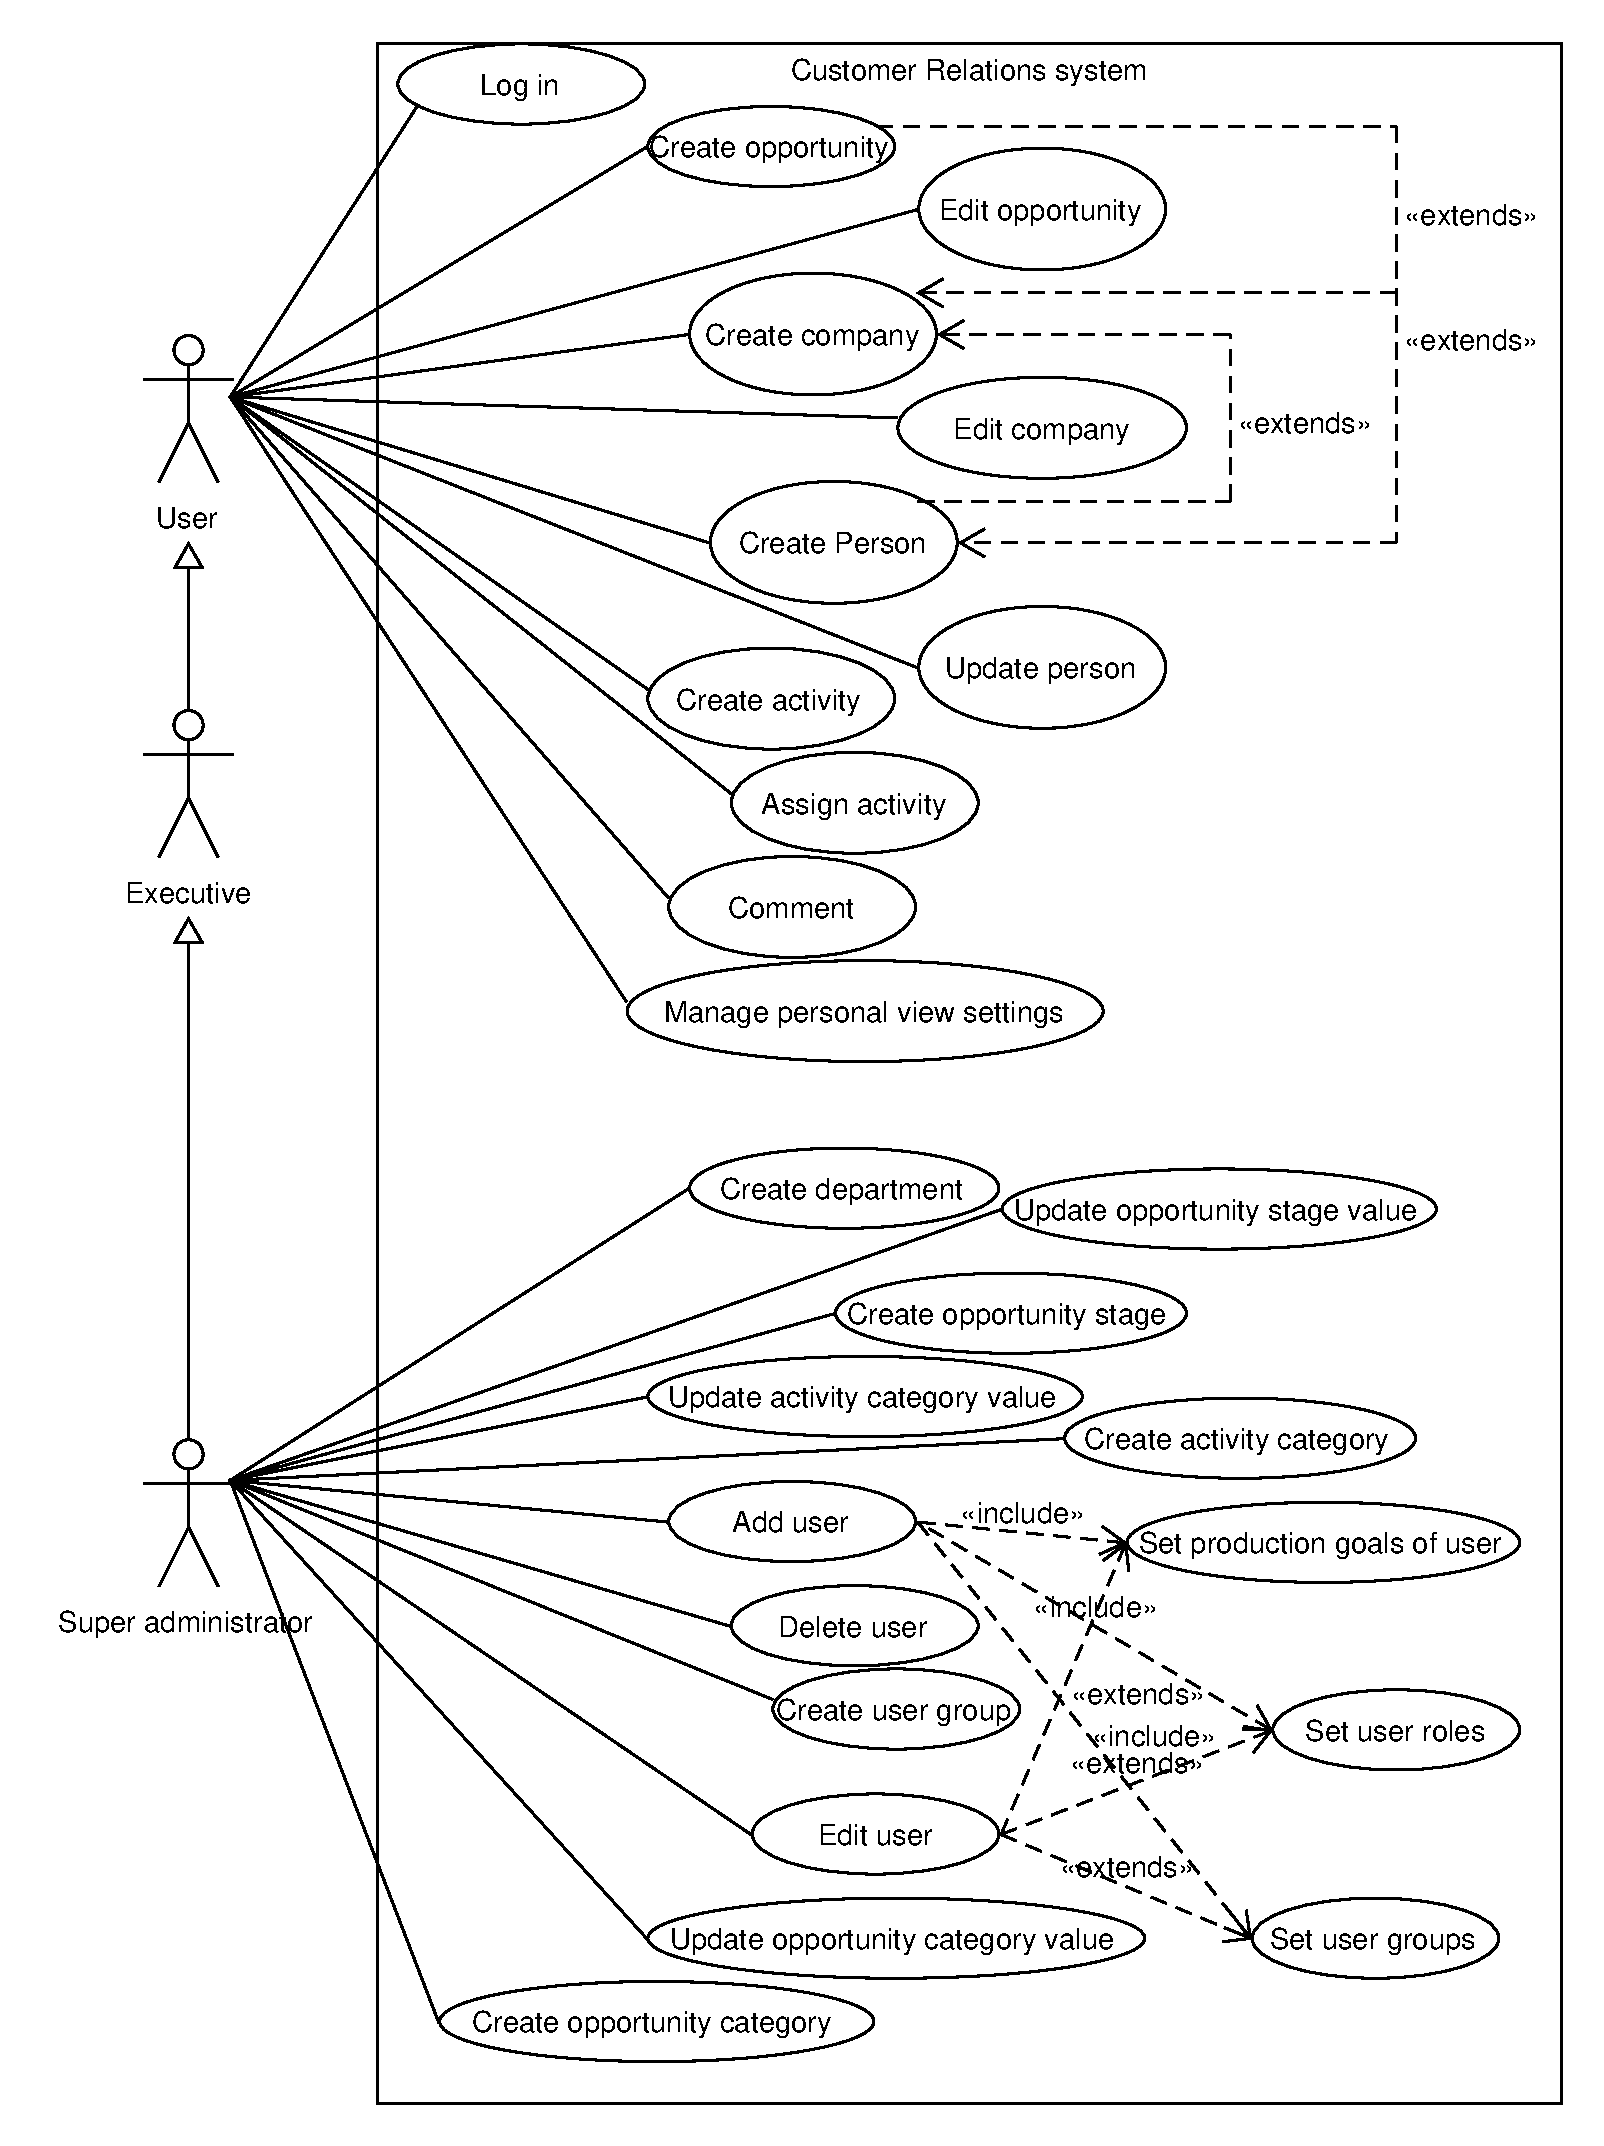
\includegraphics[width=\textwidth]{use_cases}
  \caption{Use case diagram}
  \label{fig:usecase_diagram}
\end{figure}

Because of the number of use cases in the system only a few of them have been written out fully as can be seen in the next couple of sections, the rest have a short description in appendix~\ref{app:Use cases}.

\subsection{Use case 10: Create opportunity}
\textbf{Scope}: CRM \\
\textbf{Level}: User-goal \\
\textbf{Primary actor}: User \\
\textbf{Stakeholders \& interests}:
\begin{itemize}
  \item User: Wants to be able to track the likelihood of an opportunity, and assign tasks to is, as well as keep track of opportunities in companies
\end{itemize}
\textbf{Preconditions}: User is logged in \\
\textbf{Postconditions}: Opportunity is saved. User is associated. Company associated. Person associated. Stage associated. User groups copied\\
\textbf{Main Success Scenario}:
\begin{enumerate}
  \item User fills out the Name, Description, Price, Start and End dates, Category, Hourly price, and expected close date
  \item User picks a company from a list
  \item User picks a department for the opportunity
  \item User Chooses a stage
  \item User adjusts the percentage for success
  \item User clicks save
\end{enumerate}
\textbf{Extensions}:
\begin{itemize}
  \item [1a.] User wants to add contact
  \begin{enumerate}
    \item User writes contact name
    \item List of related contacts based on company show up
    \item User selects the appropriate contact
    \begin{itemize}
      \item [3a.] User sees that the desired contact is not on the list
      \begin{enumerate}
        \item [1.] User selects create new
      \end{enumerate}
    \end{itemize}
  \end{enumerate}
  \item [2b.] Company does not exist
  \begin{enumerate}
    \item User enters company name
    \item User chooses create new
  \end{enumerate}
\end{itemize}
\textbf{Frequency of Occurrence}: Multiple times a day


\subsection{Use case 19: Create opportunity stage}
\textbf{Scope}: CRM \\
\textbf{Level}: User-goal \\
\textbf{Primary actor}: Super User \\
\textbf{Stakeholders \& interests}:
\begin{itemize}
  \item User: Wants to be able to decide on which of the created stages an opportunity should be
  \item User: Wants to get a guideline of percentage likelihood of a given stage of the sale
  \item System: Wants to be able to filter with stages
\end{itemize}
\textbf{Preconditions}: Super User is logged in \\
\textbf{Postconditions}: New stage is available. When stage is chosen the appropriate percentage is applied to opportunity.\\
\textbf{Main Success Scenario}:
\begin{enumerate}
  \item Super User clicks create new stage
  \item Super User writes a name in the name field
  \item Super User writes a value for the percentage
  \item Super User clicks save
\end{enumerate}
\textbf{Extensions}:
\begin{itemize}
  \item [4a.] System detects the name is used by another stage
  \begin{enumerate}
    \item Name field is marked as incorrect
    \item A text shows up saying the name is in use
    \item Super User chooses a different name
    \item [] Super User repeats step 4
  \end{enumerate}
\end{itemize}
\textbf{Frequency of Occurrence}: Multiple times on system setup, and adjustments

\subsection{Use case 21: Set production goals for user}
\textbf{Scope}: CRM \\
\textbf{Level}: User-goal \\
\textbf{Primary actor}: Super User \\
\textbf{Stakeholders \& interests}:
\begin{itemize}
  \item User: Wants a goal to strive for
  \item Executive and Super User: Wants to be able to get an overview of how the company is doing compared to the goals
\end{itemize}
\textbf{Preconditions}: Super User is logged in \\
\textbf{Postconditions}: The given user goals are updated from the given months and forth going. The overview compares earnings against the new goals.\\
\textbf{Main Success Scenario}:
\begin{enumerate}
  \item Super User enters edit user
  \item Super User finds the input fields for new goal at the goal list
  \item Super User chooses a month and year for the goal to run from
  \item Super User enters a value for the goal
  \item Super User clicks add
\end{enumerate}
\textbf{Extensions}:
\begin{itemize}
  \item [2a.] Super User chooses existing goal
  \begin{enumerate}
    \item Super User clicks edit
    \item [] Super User continues at step 3
  \end{enumerate}
  \item [5a.] Super User clicks update
  \item [5b.] System detects that the goal collides with another
  \begin{enumerate}
    \item Month and Year fields are marked
    \item A text shows up saying the start time for the goal is taken
    \item Super User chooses a different month or year
    \item [] Super User repeats step 5
  \end{enumerate}
\end{itemize}
\textbf{Frequency of Occurrence}: A couple of times a year for every user

\subsection{Use case matrix}
\label{sub:Use case matrix}
Based on the use cases and the requirements I have created a matrix in table~\ref{tab:Use case matrix}, showing which requirement is covered by what use case.

\begin{table}[h]
\resizebox{\linewidth}{!}{%
    \begin{tabular}{ l | *{16}{c} }
      & F1 & F2 & F3 & F4 & F5 & F6 & F7 & F8 & F9 & F10 & F11 & F12 & F13 & F14 & F15 & F16 \\
      \hline
      UC1 & X \\
      UC2 & & & X\\
      UC3 & & & X\\
      UC4 & & X\\
      UC5 & & & X\\
      UC6 & & & & & & & X & & & & & & & & & X\\
      UC7 & & & & & & & & X & & & & & & & & X\\
      UC8 & & & & & & & X & & & & & & & & & X\\
      UC9 & & & & & & & & X & & & & & & & & X\\
      UC10 & & & & & X & & & & & & & & & & X & X\\
      UC11 & & & & & & X & & & & & & & & & X & X\\
      UC12 & & & & & & & & & X & & & X & & &\\
      UC13 & & & & & & & & & & X\\
      UC14 & & & & X & & & & & & & & & X & X & X\\
      UC15 & & & & X & & & & & & & & X & X & &\\
      UC16 & & & & X & & & & & & & & X\\
      UC17 & & & & X & & & & & & & & & X & & X\\
      UC18 & & & & X & & & & & & & & & X & & X\\
      UC19 & & & & & & & & & & & & & & X\\
      UC20 & & & & X & & & & & & & & X & X & X & X\\ 
      UC21 & & & & X & & & & & & & & X & X & X & X\\
      UC22 & & & & & & & & & & & & & X & X\\
      UC23 & & & & & & & & & & & X\\
      UC24 & & X & & & & & & & & & & X & X & X & X\\
      UC25 & & & & & & & & & & & & X & X & & X\\
      UC26 & & & & & & & & & & & & & & & & X\\
      UC27 & & & & & & & & & & & & X & X & X & X\\
    \end{tabular}
}
\caption{Use case matrix showing which use cases cover what requirements}
\label{tab:Use case matrix}
\end{table}

\section{Domain Model}
\label{sec:Domain Model}
From the requirements and the use cases I can now make a domain model. The goal of this domain model is to illustrate the relations between entities in the domain\cite{larman}. This is not to say that the domain model necessarily will illustrate the actual relation between objects in the system, but rather the conceptual relation of the domain. On figure~\ref{fig:domain_model} the domain model of  the system can be seen, on the model the attributes are there because the requirements, and the use cases have shown that those are needed.

\begin{figure}[!htb]
  \centering
  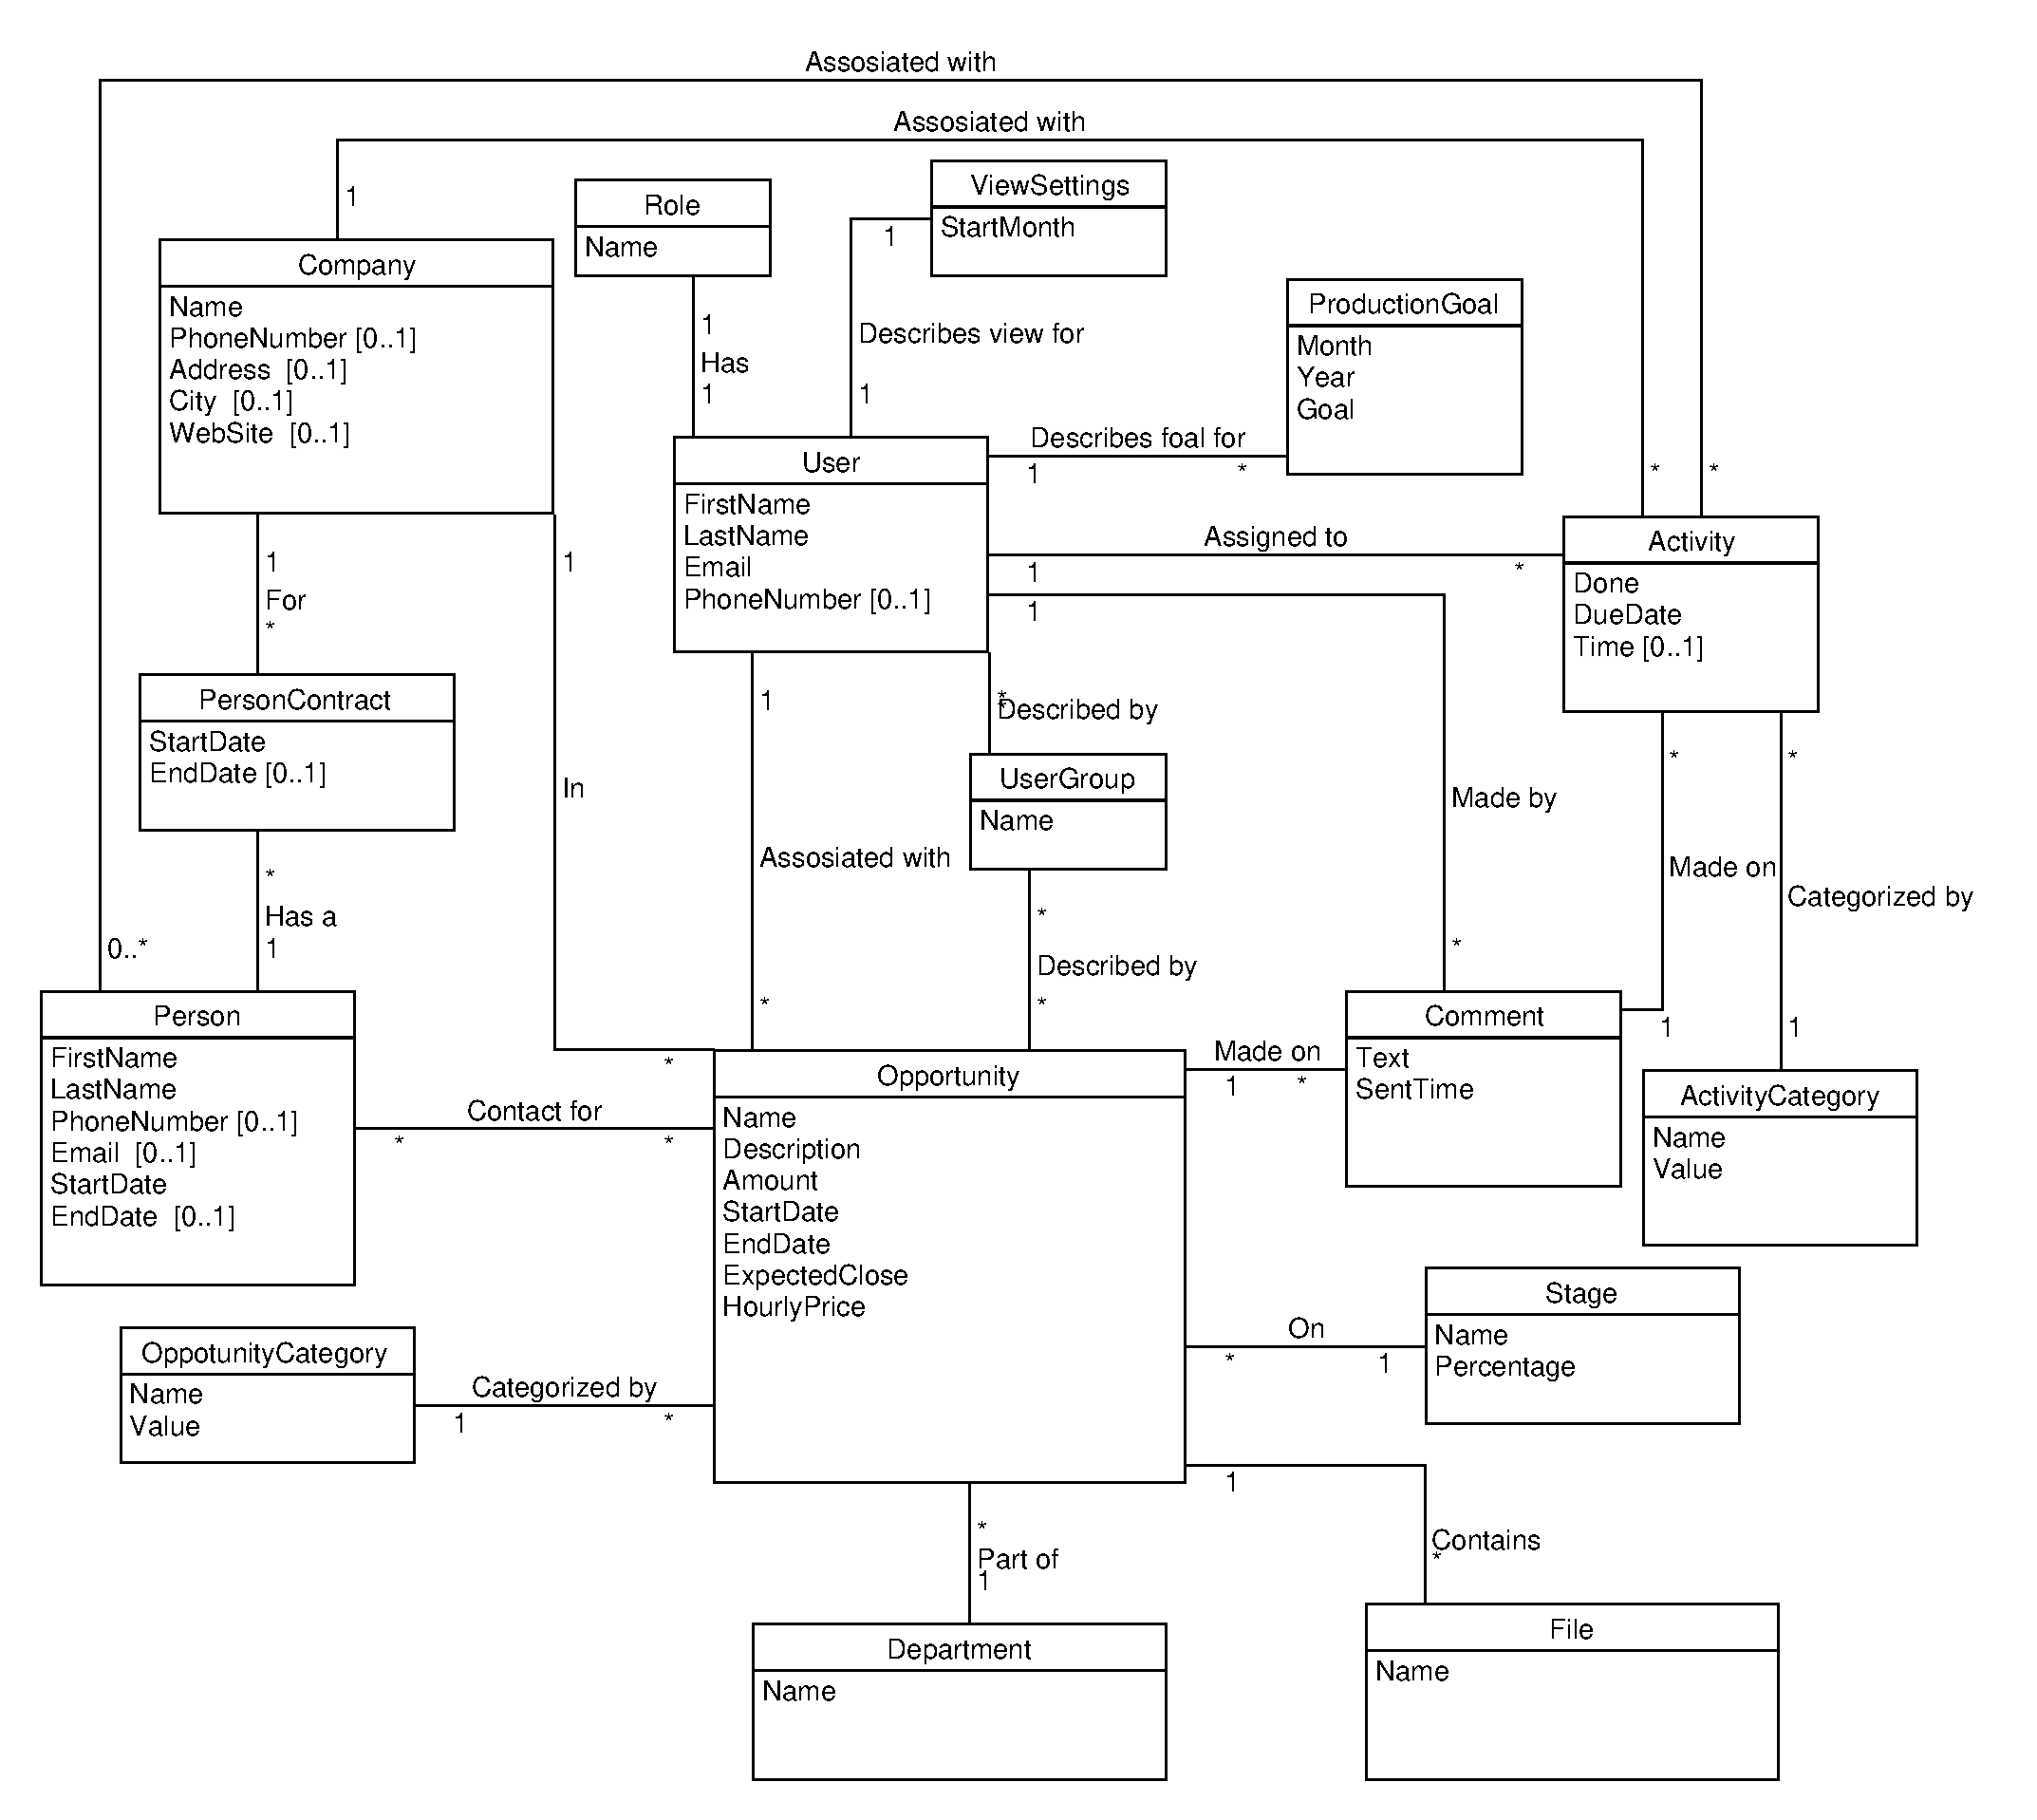
\includegraphics[width=\textwidth]{domain_model}
  \caption{Domain model}
  \label{fig:domain_model}
\end{figure}

The ranges on some of the attributes indicate if the attribute is required, so a range from 0 to 1 will indicate that it is not required.

The goal with the domain model is to increase the understanding of the system, both for the reader but also under development, allowing me to come back and look at the model, if I get unsure of how the different things are meant to relate to one another.

As can be seen in figure~\ref{fig:domain_model} the center of the system is for the most part an opportunity, which a lot of different things are connected to. Some of the connections are optional however, and can be added later, as described in the use cases. The user is also reasonably often connected to things in the model. The reason for that is given in that a user is the one who interacts with everything, both in the planning world, which is what the system partially models, and in the real world.

\section{Mockups}
\label{sec:Mockups}
Based on the use cases I have created a few mockups of some of the key parts of
the system. The goal with these mockups is not necessarily to illustrate how a
the final system would look, but more a help to imagine how a view could look,
and what information would be available in that view for it to work.

As this is a prove of concept the mockups are made from screenshots of the
system in the development phase. They started out as mockups on paper, but as it
is a prove of concept, and as such the look of the system changes a lot they
have been replaced with these.

Like I have mentioned earlier my focus is not to make a good front-end presenting
the data to the user, but rather make the backing server serving the data for
any given front-end to hook up to. I will however be making a suggestion of a
front-end, mostly to show the features of the back-end in action. This does
 mean that the mockups are not necessarily going to be representative of
a final product, and they are not meant as anything other than a help to
imagine the way the system could look. 

\begin{figure}[!htb]
  \centering
  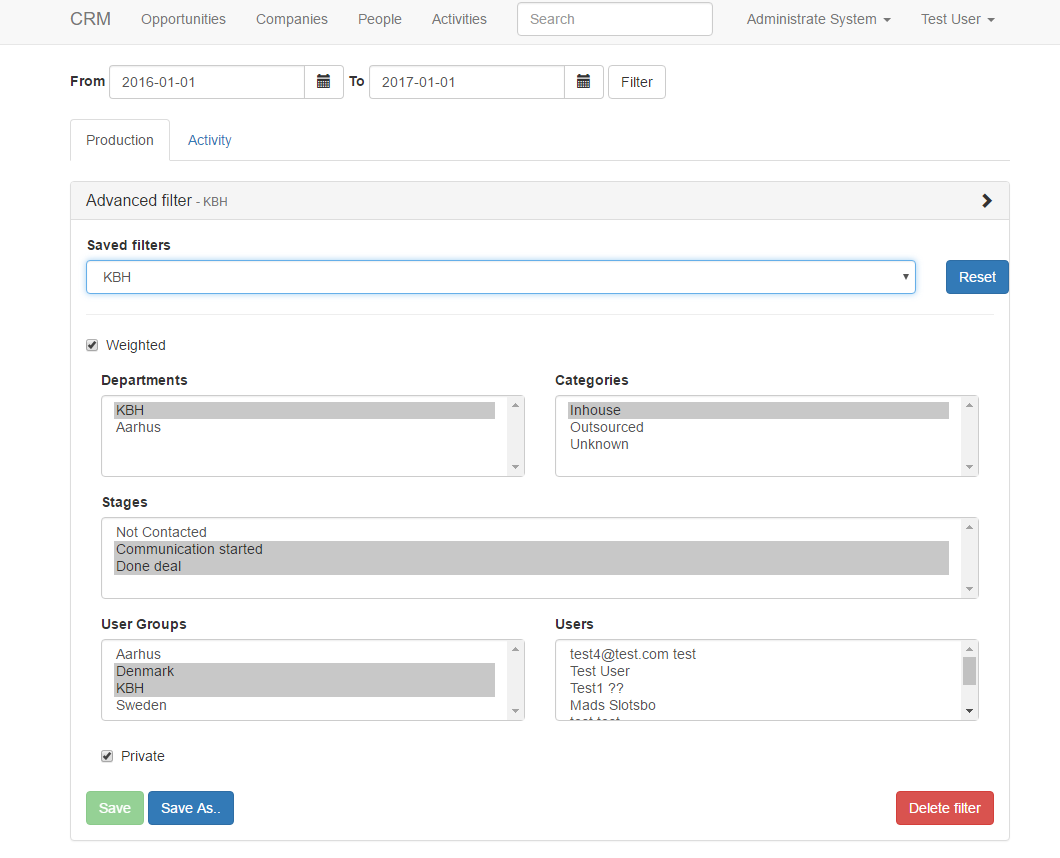
\includegraphics[width=\textwidth]{Mockups/screen_shots/filter}
  \caption{Visualization filter mockup}
  \label{fig:VisualizationFilter}
\end{figure}

\begin{figure}[!htb]
  \centering
  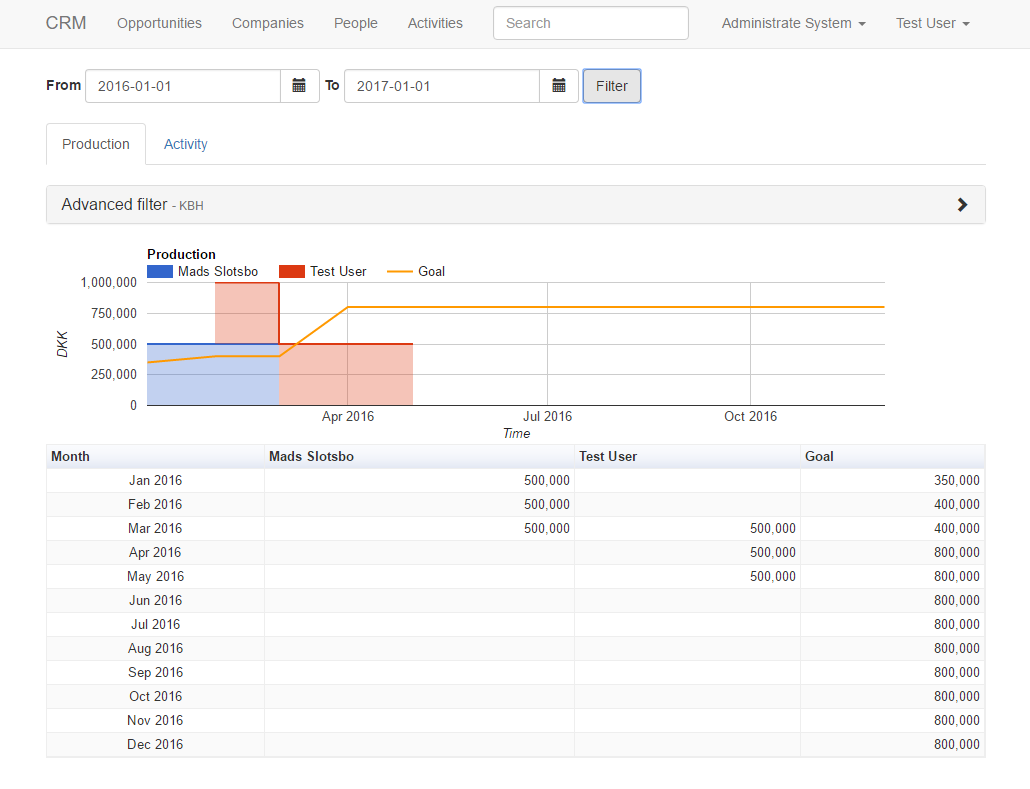
\includegraphics[width=\textwidth]{Mockups/screen_shots/graph}
  \caption{Visualization graph mockup}
  \label{fig:VisualizationView}
\end{figure}

In figure~\ref{fig:VisualizationFilter} I only show parts  of the actual view,
since underneath the folded out filter settings a graph and table similar to the
one on figure~\ref{fig:VisualizationView} would be. The idea of the mockup in
figure~\ref{fig:VisualizationFilter} is to show the filter options that a user
can apply in order for them to gain access to exactly the information they need
from this graph. This mockup is an illustration of
\nameref{app:usecase:viewsettings} as can be seen in
appendix~\ref{app:usecase:viewsettings}, and
\nameref{app:usecase:visualizegoalsproduction} from
appendix~\ref{app:usecase:visualizegoalsproduction} is represented in figure~\ref{fig:VisualizationView}

It can be seen that there are save buttons and a drop-down with names, this is to
allow the user to save a filter that they use a lot, as well as allow the admins
to set up some defaults for the users to use if they want.

\begin{figure}[!htb]
  \centering
  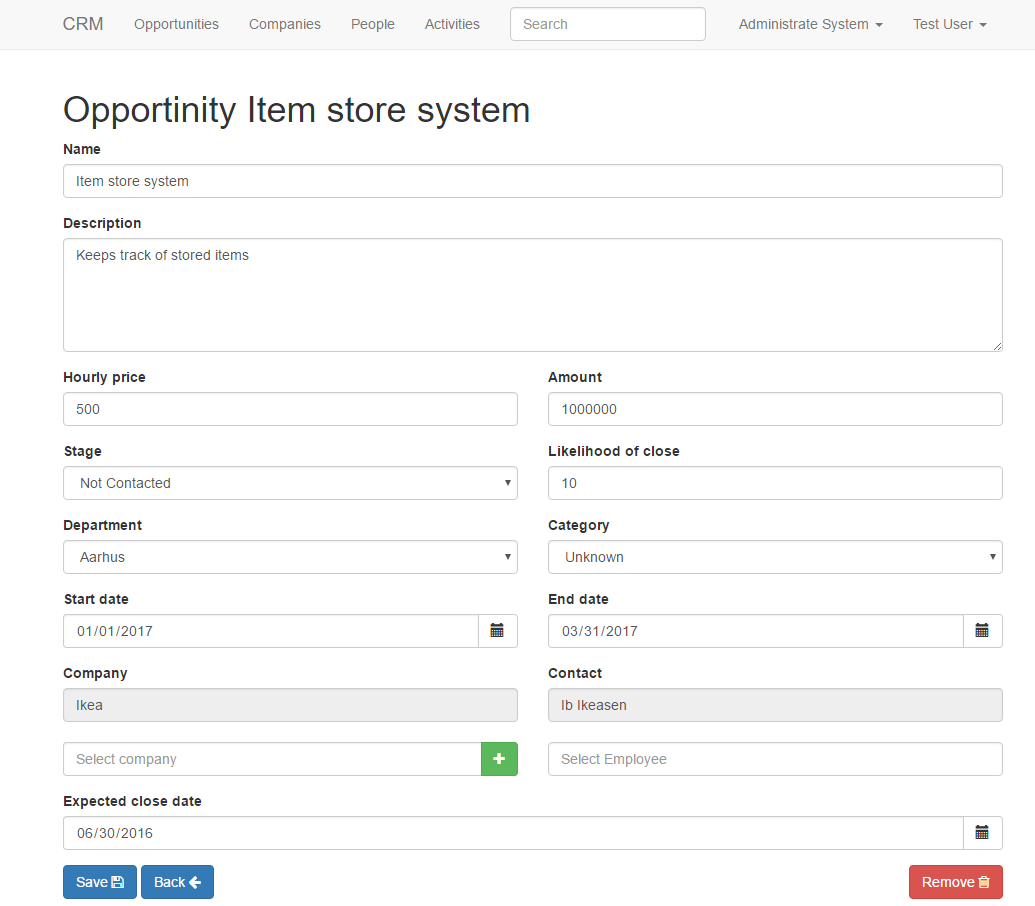
\includegraphics[width=\textwidth]{Mockups/screen_shots/edit_opportunity}
  \caption{Edit opportunity mockup}
  \label{fig:OpportunityView}
\end{figure}

\begin{figure}[!htb]
  \centering
  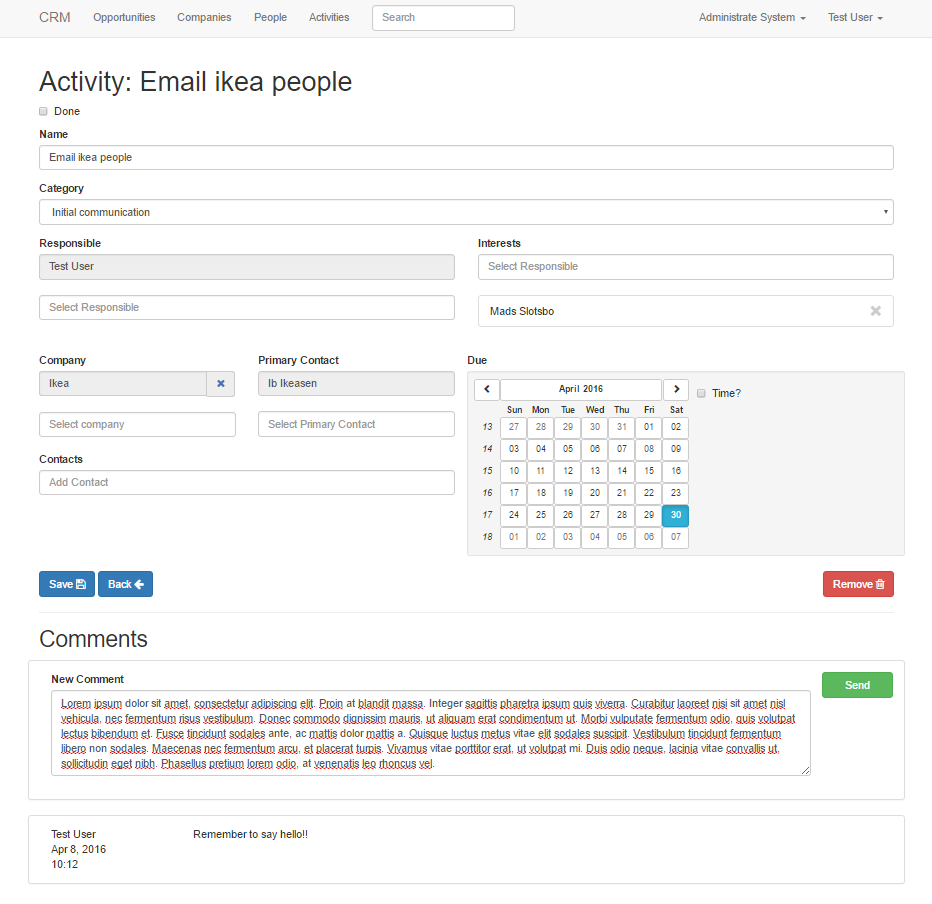
\includegraphics[width=\textwidth]{Mockups/screen_shots/edit_activity}
  \caption{Edit activity mockup}
  \label{fig:ActivityView}
\end{figure}

The two other mockups in figure~\ref{fig:OpportunityView} and
\ref{fig:ActivityView} are of some fairly essential parts of the system, namely
the management of an opportunity which is what the users will use to keep track
of tasks they may or may not win for the company. The use case where the view is
used is explained in \nameref{app:usecase:editopportunity} in
appendix~\ref{app:usecase:editopportunity} and
\nameref{app:usecase:editactivity} in appendix~\ref{app:usecase:editactivity}.


For both the contact field is
not required, but it can be used for the users to keep track of who they need to
talk to in relation to the thing they are looking at.

The mockup in figure~\ref{fig:ActivityView} has a comment section in the bottom
which is meant to be used as a way for the users to put recaps of the activity,
or maybe just notes that they need to remember in relation with it. A less
important feature is the same thing for the opportunity view, because it is not
as important for the system I have not added it in the mockup, but it would
probably end up looking a lot like the one in figure~\ref{fig:ActivityView}. 

To navigate around on the page one would follow the routes described in the
navigation diagram in figure~\ref{fig:navigation_diagram}. A thing to note about
the figure is that the main page is something that is always available, so
anything coming directly from that can be accessed from anywhere. With the
exception of activate account, as that is only linked to by an email sent to the
user on creation of a new user.

The notes are to indicate the authorization level a user needs to be able to
access that particular branch and all the nodes and sub nodes underneath.

\begin{figure}[!htb]
  \centering
  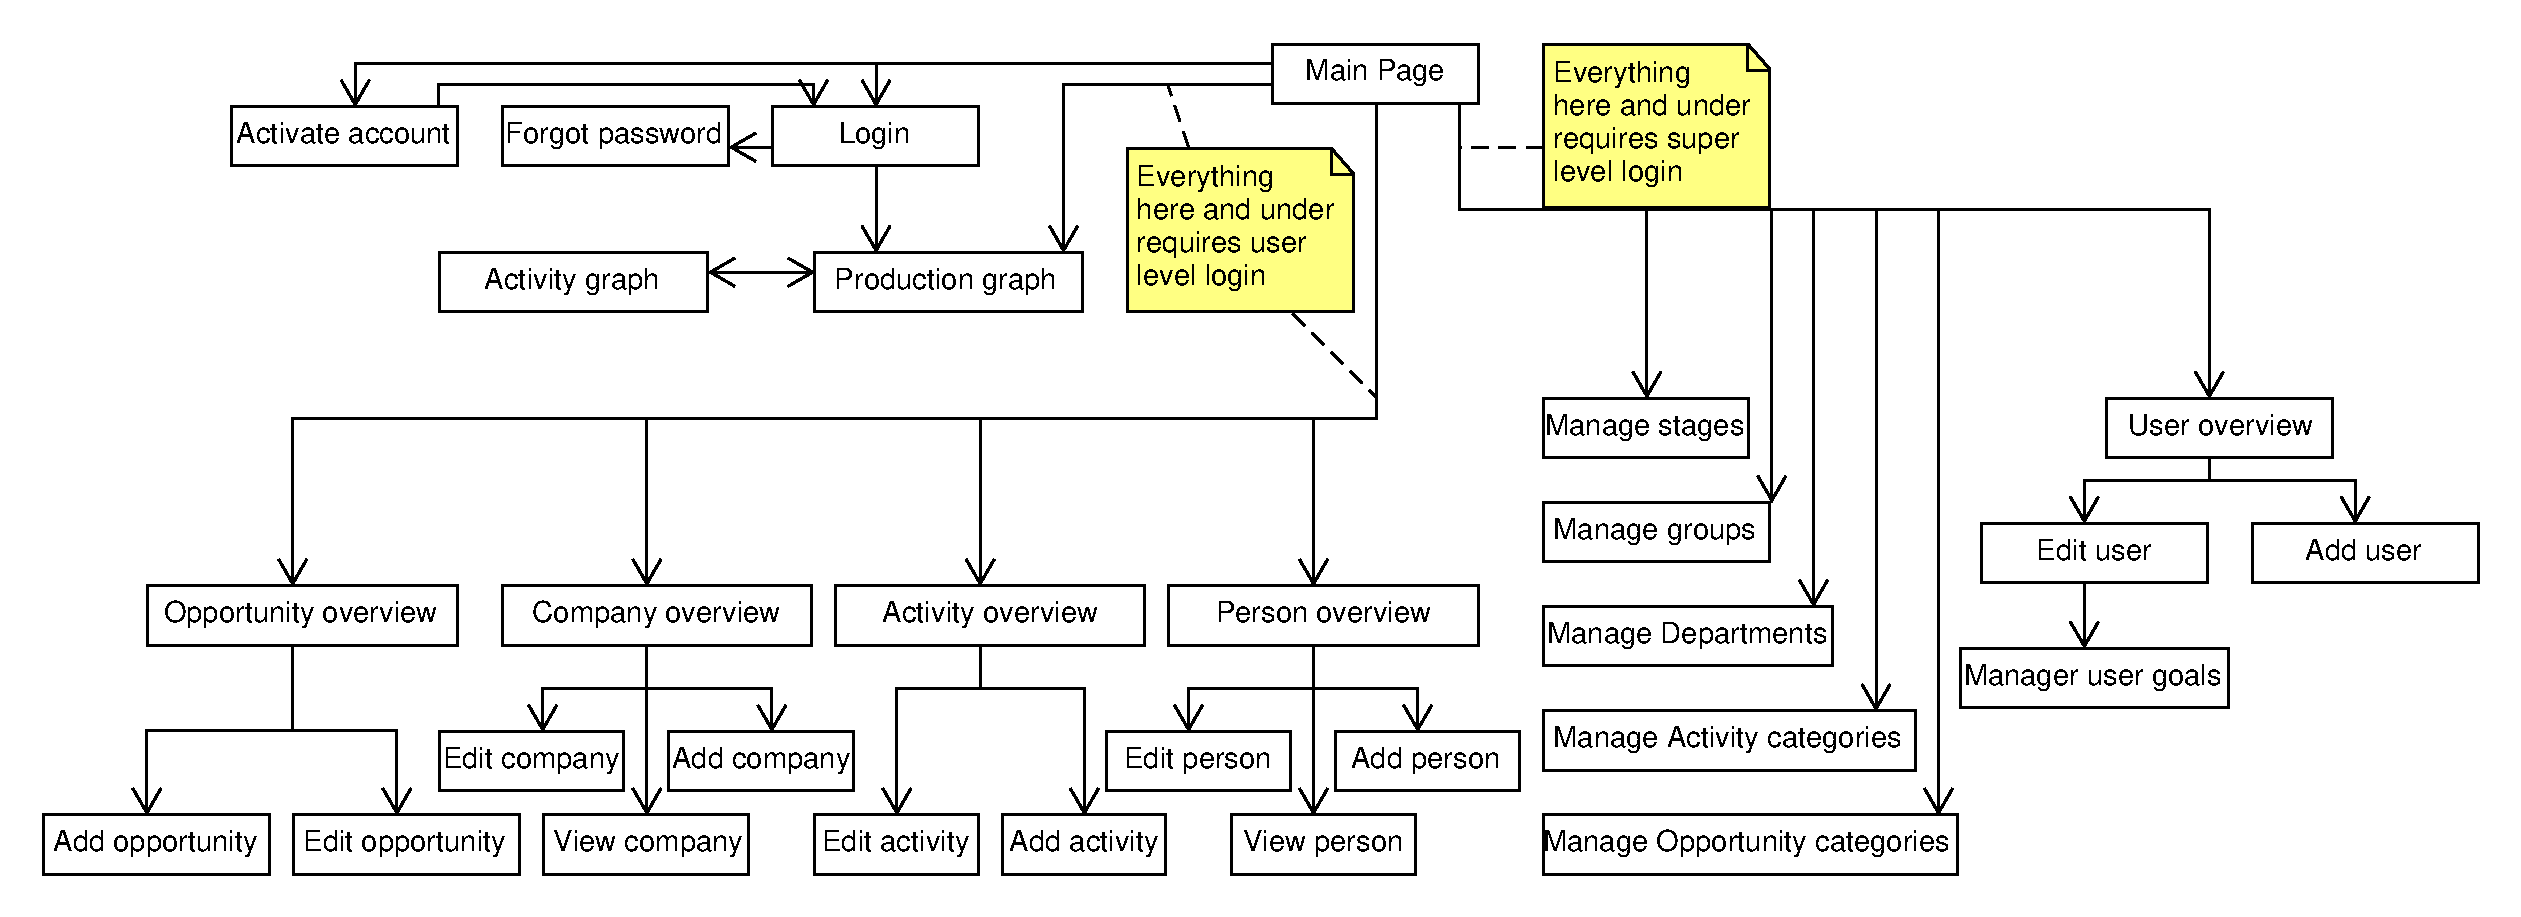
\includegraphics[width=\textwidth]{navigation_diagram}
  \caption{Navigation diagram}
  \label{fig:navigation_diagram}
\end{figure}

\section{Chapter summary}
In the system we will have 3 types of users, the standard user, an executive,
which will have no specific abilities over the standard user to begin with, but
in the future it may be needed. And finally a super user, who will be
administrating the system, creating options for drop-downs, inviting new users
and the like.

One of the things the super user is meant to do is to customize the system by
setting categories, goals, and groups. Another thing that is important for the system,
is the ability to get an overview so that a user can know how they are doing, or
how the company is doing. This should be made in a way so that it can easily be
graphed.
